\section{实值函数及其界}
\label{sec:real-valued-functions-bounds}

第~\ref{chap:sets-relations-maps}章的映射可以取值于任意集合。本章研究的数列与函数都取实数值，
实数既能相加相乘，又能比较大小：前者使函数之间可以逐点运算，后者引出“能取到多小的值”这类问题。
极限存在与否，最终也要回到实数集合有没有最小的上界。本节先说明实值函数的逐点运算，
再把整个函数作为集合的元素，讨论用参数编号的函数族；最后建立实数集合的确界、实数的完备性与函数的最值，
它们是下一节判断极限存在的依据。

\subsection{实值函数的运算}
\label{sec:real-function-arithmetic}

若$f,g:X\to\mathbb R$有相同定义域，可以在每个输入处计算函数值的和、差、积：
\[
 \begin{aligned}
 (f+g)(x)&=f(x)+g(x),\\
 (f-g)(x)&=f(x)-g(x),\\
 (fg)(x)&=f(x)g(x).
 \end{aligned}
\]
对实常数$c$，定义
\[
  (cf)(x)=cf(x).
\]
这些新函数的定义域仍是$X$。

商函数则只在分母不为零的范围内定义：
\[
  (f/g)(x)=f(x)/g(x),
\]
其定义域为$\{x\in X:g(x)\neq0\}$。例如在$\mathbb R$上取$f(x)=x$、$g(x)=x-1$，则$(f+g)(x)=2x-1$定义在整个实轴上，
而$(f/g)(x)=x/(x-1)$的定义域不含$1$。
与复合不同，逐点运算要求两个函数有相同的定义域，并在每个输入处对两个函数值做实数运算；
复合则把一个函数的输出作为另一个函数的输入，见第~\ref{sec:prelim-map-operations}节。

\subsection{函数族与参数化}
\label{sec:prelim-function-families}

\paragraph{函数族}
设想由输入预测输出：事先并不知道哪条规则最合适，通常先划定一批候选规则，再从中挑选。
这批候选规则本身是一个集合，它的元素是整个函数。
具有同一定义域和陪域的一组函数组成函数族（family of functions）。

例如，形如$f(x)=ax+b$的函数称为一元仿射函数（affine function），所有这样的函数组成
\[
 \mathcal F=\{f_{a,b}:\mathbb R\to\mathbb R:\ f_{a,b}(x)=ax+b,\ (a,b)\in\mathbb R^2\}.
\]
族中的每个元素是一整个函数。取$(a,b)=(2,1)$得到函数$f_{2,1}(x)=2x+1$；
再取输入$x=3$，才得到一个函数值$f_{2,1}(3)=7$。

\paragraph{函数参数化}
用参数为函数族中的函数编号，称为参数化（parameterization）。
一般写成$\theta\mapsto f_\theta$，其中$\theta$属于参数集合$\Theta$，
$f_\theta:X\to Y$是相应的函数。
映射$\theta\mapsto f_\theta$的输入是参数，输出是函数；函数$f_\theta$自身的输入仍是$x$。
在上例中，$\theta=(a,b)$指定一条直线，而$x$指定在直线上的哪个位置求值。
参数化把“在函数中挑选”改写为“在参数集合中挑选”；参数集合通常是$\mathbb R^2$这样熟悉的集合，
便于后续用数值方法比较和调整。

\paragraph{函数参数化的可识别性}
不同参数可能表示同一个函数，所以参数与函数未必一一对应。能否由函数反过来确定参数，取决于下面的条件。
\begin{definition}[函数参数化的可识别性]
\label{def:prelim-identifiable-parameterization}
给定参数集合$\Theta$与函数族$\{f_\theta:X\to Y:\theta\in\Theta\}$。
若$f_\theta=f_{\theta'}$蕴含$\theta=\theta'$，即$\theta\mapsto f_\theta$为单射，
则称这一函数参数化可识别（identifiable）；也就是说，完整函数唯一确定其参数。
否则称为不可识别。
\end{definition}
这里比较的是整个定义域上的函数，而非几个位置的函数值。
例如仿射函数族中$b=f_{a,b}(0)$、$a=f_{a,b}(1)-f_{a,b}(0)$，
所以完整函数唯一确定$(a,b)$，这一参数化可识别。若只观察$x=0$处的函数值，则只能确定$b$，
不能确定$a$。可见，有限个观测是否足以确定参数，与参数化是否可识别是两个不同的问题。

\Needspace{11\baselineskip}
\begin{example}[参数不同而函数相同]
\label{ex:prelim-nonidentifiable-parameterization}
考虑参数化函数
\[
  f_{a,b}:\mathbb{R}\to\mathbb{R},
  \qquad
  f_{a,b}(x)=abx,
  \qquad
  (a,b)\in\mathbb{R}^2.
\]
参数$(1,2)$与$(2,1)$不同，却对每个$x$给出相同的函数值。更一般地，只要$c\neq0$，
$(ca,b/c)$与$(a,b)$就表示同一个函数。从完整的输入输出关系可以确定乘积$ab$（例如取$x=1$，有$ab=f_{a,b}(1)$），
却不能分别确定$a$和$b$。这是参数化本身不可识别，而不是计算精度不足。
\end{example}


图~\ref{fig:vol1-add-parameter-function-value}把“由参数得到函数”和“由函数得到函数值”这两层操作分开：三组不同参数先汇入同一条完整规则，然后才在指定的$x$处求值。
\begin{figure}[!htb]
  \centering
  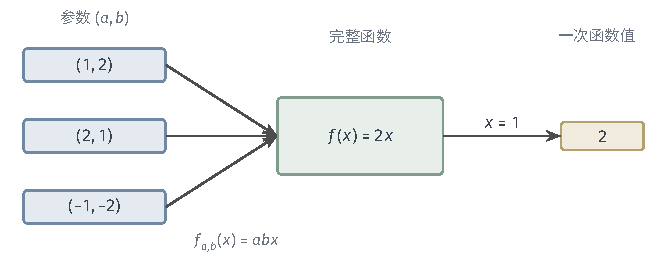
\includegraphics[width=112mm]{figures/01-mathematical-preliminaries-upper/00-shared/tikz/mathematical-language-combinatorics-analysis-optimization-comprehension-additions/parameter-function-value.pdf}
  \caption{参数化$f_{a,b}(x)=abx$中的三层对象。参数$(1,2),(2,1),(-1,-2)$的乘积均为$2$，所以它们表示同一个函数$f(x)=2x$；再指定$x=1$，才得到一次求值结果$2$。多组参数汇入同一完整函数，正是不可识别性。}
  \label{fig:vol1-add-parameter-function-value}
\end{figure}

不可识别的参数可以用第~\ref{sec:prelim-equivalence-relations}节的等价关系整理。规定$\theta\sim\theta'$当且仅当$f_\theta=f_{\theta'}$，
就得到参数集合上的等价关系：函数相等本身是反身、对称、传递的，三条性质直接继承。
每个等价类收集同一个函数的全部参数表示；在$f_{a,b}(x)=abx$中，$(a,b)$所在的等价类是满足$a'b'=ab$的全部参数$(a',b')$。

把每个等价类对应到它所表示的函数，就得到从商集$\Theta/{\sim}$到函数族$\{f_\theta:\theta\in\Theta\}$的双射。
参数化可识别，恰好意味着每个等价类只含一个参数。
换言之，函数族中的元素按函数区分，参数则可能为同一个函数保留多种表示。

\subsection{实值函数的界与极值}
\label{sec:prelim-optimal-values-errors}

从候选函数中挑选时，常把每个候选的优劣写成一个实数，例如预测误差，再寻找使它最小的候选。
这就要求讨论一个实值函数能取到多小的值、最小值是否真的取得。
函数值组成实数集合，而实数的通常大小$\leq$是全序。下面先把偏序集合中的界用于实数并定义确界，
说明保证确界存在的实数完备性，再把这些概念用于函数。

\paragraph{上界与下界}
设$A\subseteq\mathbb R$非空。若$a\leq M$对每个$a\in A$成立，
就称$M$为$A$的上界（upper bound）；若$m\leq a$对每个$a\in A$成立，
就称$m$为下界（lower bound）。这正是第~\ref{sec:prelim-order-relations}节偏序集合中上界、下界的定义在$(\mathbb R,\leq)$中的情形。
存在上界称为上有界，存在下界称为下有界，两者都有称为有界。
例如$(0,1)$有上界$1,2$，也有下界$0,-1$。界不必是集合中的元素，也不唯一。

\paragraph{上确界与下确界}
上界中的最小者称为\term{上确界}（supremum），记作$\sup A$；
下界中的最大者称为\term{下确界}（infimum），记作$\inf A$。
例如$\sup(0,1)=1$、$\inf(0,1)=0$，两个确界都不属于$(0,1)$。

上确界$\beta$不仅要满足$a\leq\beta$对所有$a\in A$成立，
还要满足每个$\varepsilon>0$都存在$a\in A$使$a>\beta-\varepsilon$。
后一个条件说明，任何比$\beta$小的数都不是上界。
下确界$\alpha$类似地满足$\alpha\leq a$对所有$a\in A$成立，且每个$\varepsilon>0$都存在$a\in A$
使$a<\alpha+\varepsilon$。

上界有无限多个，其中是否真有最小的一个，并不能从定义直接看出。
本书把下面的性质作为实数的基本性质使用，称为实数的完备性（也称确界原理）：
非空上有界实数集合有实数上确界，非空下有界实数集合有实数下确界。
有理数没有这一性质：集合$\{q\in\mathbb Q:q^2<2\}$在有理数中有上界（例如$2$），
但它在实数中的上确界是$\sqrt2$，而$\sqrt2$不是有理数。于是每个有理上界都严格大于$\sqrt2$，
在它与$\sqrt2$之间总还有更小的有理上界，所以在有理数中找不到最小的上界。
实数补上了这样的“空隙”，后面关于极限存在的结论都要用到这一点。

\paragraph{函数的有界性}
对非空定义域$X$上的实值函数$f:X\to\mathbb R$，讨论其有界性就是讨论值域$f(X)$的有界性。
例如$f(x)=x$在$(0,1)$上有界，在$\mathbb R$上则既无上界也无下界。
值域的确界简记为
\[
 \inf_{x\in X}f(x)=\inf f(X),\qquad
 \sup_{x\in X}f(x)=\sup f(X).
\]
若$f(X)$无下界，约定其下确界为$-\infty$；若无上界，约定其上确界为$+\infty$。
这两个符号表示没有有限的界，不是实值函数实际取到的数。

\paragraph{最小值与最小点}
若存在$x^\star\in X$使
\[
 \forall x\in X,\qquad f(x^\star)\leq f(x),
\]
则称$x^\star$为\term{全局最小点}（global minimizer），$f(x^\star)$为最小值。
符号$\forall$读作“对所有”，这里要求与定义域内的每个函数值比较。
最小值记作$\min_{x\in X}f(x)$；全部最小点组成的集合记作
\[
 \argmin_{x\in X}f(x)
 =\{x\in X:\ f(x)\leq f(z)\text{ 对所有 }z\in X\}.
\]
$\min$给出一个数，$\argmin$给出输入的集合；若不存在最小点，后一个集合为空。

最小值存在时必等于下确界：$f(x^\star)$不超过每个函数值，所以是值域的一个下界；
任何下界$m$都满足$m\leq f(x^\star)$，因为$f(x^\star)$本身就是一个函数值。
所以$f(x^\star)$是最大的下界。反过来，下确界存在却未必被取得。
例如$f(x)=x$在$(0,1)$上的下确界为$0$，但没有最小点，
因为任意允许的$x$都有更小的允许输入$x/2$。

\paragraph{最大值与最大点}
若存在$x^\star\in X$使$f(x^\star)\geq f(x)$对所有$x\in X$成立，
则称$x^\star$为全局最大点，$f(x^\star)$为最大值。
最大值记作$\max_{x\in X}f(x)$，全部最大点组成
\[
 \argmax_{x\in X}f(x)
 =\{x\in X:\ f(x)\geq f(z)\text{ 对所有 }z\in X\}.
\]
与最小值的论证对称，最大值存在时等于上确界。函数$f(x)=x$在$(0,1)$上没有最大值；
将定义域换为$[0,1]$后，最大值为$1$、最大点为$1$，最小值为$0$、最小点为$0$。

\begin{example}[同一个最优值可以对应多个输入]
\label{ex:prelim-optimal-value-versus-points}
令$X=[-2,2]$，$f(x)=(x^2-1)^2$。平方非负，且$x=\pm1$都使它为零，所以
\[
  \min_{x\in X}f(x)=\inf_{x\in X}f(x)=0,\qquad
  \argmin_{x\in X}f(x)=\{-1,1\}.
\]
又因为$0\leq x^2\leq4$，有$|x^2-1|\leq3$，于是$f(x)\leq9$，等号恰在$x=\pm2$
处成立。因此最大值为$9$，最大点集合为$\{-2,2\}$。最小值是一个数，不会因为有两个
最小点就变成两个最小值；最优点是否唯一是另一个问题。
\end{example}

图~\ref{fig:prelim-minimum-infimum}固定表达式$f(x)=x$，比较它在$(0,1)$与$[0,1]$上定义的两个函数。
两侧的函数值都以$0$为下确界；右侧把$x=0$纳入定义域后，这个下确界才由某个输入取得。
区别的关键在于边界点是否属于定义域，而不在于两条曲线是否趋向同一个高度。

\begin{figure}[htbp]
  \centering
  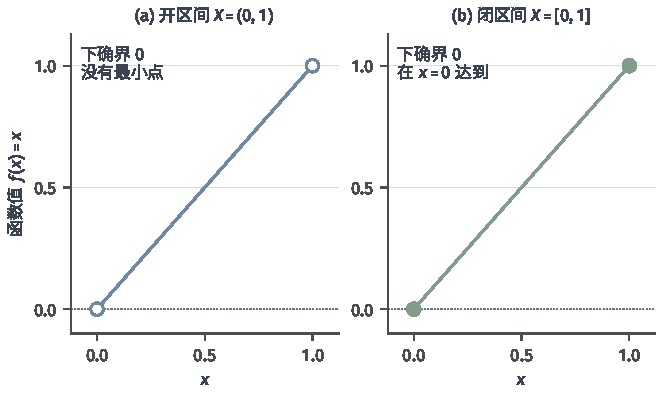
\includegraphics[width=112.0mm]{figures/01-mathematical-preliminaries-upper/01-mathematical-language-combinatorics-analysis-optimization/matplotlib/prelim-minimum-infimum/figure.pdf}
  \caption{同一求值表达式$f(x)=x$在两个定义域上的边界对照。左图定义域为$(0,1)$，空心端点不属于图像，函数值可任意接近$0$，却不能取到；右图定义域为$[0,1]$，实心端点$(0,0)$达到下确界。两图的下确界相同，最小点是否存在取决于可行端点是否保留。图为解析教学示例。}
  \label{fig:prelim-minimum-infimum}
\end{figure}
\FloatBarrier
